\documentclass[11pt]{article}
\usepackage[T1]{fontenc}
\usepackage[utf8]{inputenc}
\usepackage{comment}
\usepackage{makecell}
\usepackage{graphicx} 
\usepackage{siunitx}
\usepackage{float}
\usepackage{url}

% 1-inch margins
\usepackage[margin=1in]{geometry} 

% Double spacing
\usepackage{setspace}
\doublespacing

% Use proper Times New Roman -- requires compiler XeLaTeX
%\usepackage{fontspec}
%\setmainfont{Times New Roman}

% set Times New Roman-style font but stay with pdfLatex compiler 
%\usepackage{newtxtext}
%\usepackage{newtxmath}
\usepackage[scaled]{helvet}
\renewcommand{\familydefault}{\sfdefault}
%\usepackage{sansmath}
%\sansmath
% For basic formatting
\usepackage{graphicx}
\usepackage{amsmath, amssymb}

% Optional: hyperlinks in references or text
%\usepackage[colorlinks=true, linkcolor=blue, parencitecolor=blue, urlcolor=blue]{hyperref}

% Page number in header
\usepackage{fancyhdr}
\pagestyle{fancy}
\fancyhf{}
\rhead{\thepage}
\renewcommand{\headrulewidth}{0pt}

% Paragraph formatting per APA
\setlength{\parindent}{0.5in}
\setlength{\parskip}{0pt}

% citations - APA 7
%\usepackage[backend=biber,style=apa]{biblatex}
\usepackage[style=apa,sorting=nyt,hyperref=true]{biblatex} % referencing. nyt = name, year, title
\addbibresource{bib.bib}

\begin{document} 


\title{A problem that should not be skipped: How non-attempts interfere with tracking abilities in adaptive learning systems}
% Disentangling response processes in adaptive learning systems: ..
% When metacognitive processes ..
% How non-attempts interfere with tracking abilities in adaptive learning systems
% Tracking learner abilities with confidence: ..
% A problem that should not be skipped: How non-attempts bias adaptive learning systems

% A problem that should not be skipped: Disentangling skips from errors in adaptive learning systems
% A problem that should not be skipped: How non-attempts interfere with tracking abilities in adaptive learning technologies 
% Beyond blank responses: Accounting for non-attempts in adaptive learning technologies 
% Making skips count: ...
\date{}
\maketitle


\begin{abstract}
Adaptive learning systems often experience non-attempts, such as skipping problems. This behavior is usually intentionally permitted to sustain motivation, enable self-regulation, and bypass poorly matched problems. However, offering explicit options for non-attempts can have desirable and undesirable metacognitive effects, ranging from self-regulation to effort avoidance or gaming the system. Importantly, these metacognitive effects may invalidate the unidimensionality assumption underlying some measurement models in adaptive systems. This can limit the accuracy and fairness of ability estimates, ultimately lowering the system's effectiveness. In this study, we apply a tree-based item response model to disentangle cognitive ability from non-attempt behavior, using data from over \num{3500} learners from a large-scale K-12 adaptive learning platform. We find that ability and non-attempt are moderately correlated, but distinguishable latent traits, confirming that non-attempts should not be ignored when estimating learner ability. These results highlight a core tension in adaptive educational technology design: powerful unidimensional models offer practical efficiency, but more complex models may be needed to capture individual differences in metacognitive processes. We discuss implications for both measurement practice and platform design, and propose several ways to navigate this trade-off. 
 
\end{abstract}

\paragraph{Keywords}
adaptive learning, learner performance modeling, problem-skipping, item response tree, K-12 education, fairness
\newpage 

\section{Introduction}
% 1. Problem setting (one or two paragraphs, this should set the broader BJET tone for the article)
% - Set importance: One of the main promises of large-scale online learning systems is personalization. There are now many such systems used by many users worldwide. Unidimensional models have shown to be promising for reason a b c.
% - Empirical fact/phenomenon: Online learning systems often exhibit significant non-response (few quick refs).
% - Causes: Intentional option for this with good reasons (name them and ref).
% - Consequences for student behavior: Enables additional metacognitive strategies, both desirable and undesirable.
% - Consequences for measurement/personalization: metacognitive behavior can be a direct threat to the promise of accurate personalization, affecting those many users.

Adaptive learning systems (ALS) are increasingly used to support personalized instruction in digital learning environments~\parencite{vanlehn2011relative, walkington2013using, jiang2023fly}. By continuously adjusting the difficulty of tasks to match a learner's current level of understanding, such systems aim to provide practice that is neither too easy nor too difficult, effectively keeping learning inside the zone of proximal development~\parencite{vygotsky1978mind}. To accomplish this, adaptive platforms rely on statistical models that estimate a learner's current proficiency based on their observed performance during practice (\textit{i.e.,} a student model). Item response theory (IRT) models are commonly used for this purpose: they produce interpretable estimates of learner ability that scale efficiently to large student populations, and update continuously as learners practice~\parencite{rasch1993probabilistic, klinkenberg2011computer, weiss1982improving, jiang2023fly}. The accuracy of these estimates directly determine how effectively practice can be personalized.

At the same time, many digital learning environments offer ways to respond beyond simply answering a question. Studies of large-scale platforms report that a substantial proportion of responses involve skipping or help requests rather than genuine attempts~\parencite{castro2015building, wang2011assistance, savi2018delaying, savi2023combating, gorgun2022considering}. Such non-attempt options are often included as a response option intentionally, for example to reduce frustration~\parencite{fidan2024emotions}, maintain engagement~\parencite{savi2018delaying}, support metacognitive self-regulation~\parencite{roll2015understanding}, or prevent learners from getting stuck~\parencite{aleven2000limitations}. Yet non-attempt behavior does not lend itself to a single interpretation. It may reflect productive metacognitive strategies, such as recognizing the limits of one's knowledge or seeking guidance when stuck~\parencite{fleur2021metacognition, shields2024active}. Equally, it may reflect unproductive behaviors such as effort avoidance~\parencite{savi2023combating} or gaming the system~\parencite{baker2004off}---bypassing difficult problems rather than engaging with them. This complicates interpretation of the student model, which assumes that observed behavior is a reflection of task proficiency alone, threatening both the accuracy and fairness of personalization at scale.

In this study, we apply an IRTree model to data from a large-scale adaptive learning platform to test whether non-attempt behavior and task proficiency constitute distinguishable latent traits, and examine how the two processes relate.
 
% "Attempts": https://files.eric.ed.gov/fulltext/ED560903.pdf, https://www.researchgate.net/publication/221438300_The_Assistance_Model_Leveraging_How_Many_Hints_and_Attempts_a_Student_Needs
%Statistical models continuously update these ability estimates, which simultaneously guide the selection of subsequent tasks. 
%At the same time, many digital learning environments offer ways to respond beyond simply answering a question. Learners may request hints (ref), skip items (ref), or indicate that they do not know the answer (ref). Such a response allows the student to avoid attempting the problem; we therefore refer to this response behavior as a non-attempt. Non-attempt options are often included to support productive learning strategies, reduce frustration, or maintain engagement during practice. However, they also introduce multiple behavioral pathways through which learners can interact with a task. When learners choose to skip a problem or request help rather than attempt a response, their behavior may reflect metacognitive regulation, strategic effort allocation, or disengagement rather than task proficiency alone. This raises an important question for adaptive learning systems: should such behaviors be interpreted separately from learner ability? 

\subsection{Unidimensional measurement models}
% Adaptive learning systems rely on a student model -- needs psychometrics -- common approach is irt -- rasch model is one formulation -- give formula -- explain person and item params 
The main goal of an ALS is to continuously update a learner's proficiency in order to match them to appropriate tasks. Central to this process is the student model: a statistical representation of what a learner knows at a given point in time, inferred from their observed responses, and updated as new responses come in~\parencite{corbett1994knowledge, deonovic2018learning, klinkenberg2011computer}. Building and maintaining this model requires psychometric methods that can translate observed responses into latent ability estimates. A widely used psychometric framework for student modeling is item response theory~\parencite[IRT;][]{hambleton1991fundamentals}, which has proven particularly useful when applied in large-scale adaptive contexts~\parencite{pelanek2016applications}. In IRT, learner- and item characteristics are estimated as parameters on a shared latent scale, allowing the direct comparison of a learner's ability against an item's difficulty. A simple and commonly used formulation is the Rasch model~\parencite{rasch1993probabilistic}, where the probability that person \textit{p} answers item \textit{i} correctly is a function of these two quantities:

\begin{equation}
P(X_{pi} = 1 \mid \theta_p, \beta_i) = \frac{e^{(\theta_p - \beta_i)}}{1 + e^{(\theta_p - \beta_i)}},
\label{eq:Rasch}
\end{equation}

\noindent where the ability parameter $\theta_p$ represents how proficient the learner is relative to the item pool, and the item difficulty parameter $\beta_i$ represents the ability level at which a learner has a 50\% chance of answering the item correctly. In ALS, both parameters are updated while learners interact with the system~\parencite[for example with the Elo-algorithm; ][]{klinkenberg2011computer}, giving the system a continuously refined estimate of proficiency. Crucially, both parameters occupy a single latent dimension. Thus, the student model is unidimensional and performance is assumed to be driven by a single latent dimension.

% Advantages of unidimensionality 
This property has had major advantages for educational technology, with IRT-based adaptive systems now serving millions of learners worldwide~\parencite{brinkhuis2018learning, pelanek2016applications, settles2020machine}. Because ability and difficulty are on the same scale, items can be dynamically selected to match a learner's current estimated proficiency~\parencite{weiss1982improving, magis2017computerized}. Under the assumptions of the student model, the framework is also measurement-invariant: ability estimates do not depend on which particular items a learner encounters, enabling fair comparison across learners who engage with different subsets of an item pool~\parencite{rasch1993probabilistic, wright1982rating}. These properties support a range of practical applications — from teacher-facing progress monitoring and mastery management~\parencite{maris2012speed, deonovic2018learning, saric-grgic2024twenty-five} to improved learning efficiency and sustained engagement for students~\parencite{eggen2006optimal, ma2014intelligent}.

% Risks of unidimensionality 
Although unidimensional student models appear powerful for education, their advantages rest on the critical assumption that the observable performance is truly unidimensional. If response behaviors are driven by processes other than proficiency, unidimensional models may conflate distinct sources of variability, potentially conflating both person and item estimates. This is a particular concern in adaptive practice contexts, where learners can avoid attempting a problem, possibly resulting in a second dimension next to performance. For example, independent of the ability of two students, one may skip because they correctly judge that they do not know the answer, whereas another may skip simply to avoid the effort of responding~\parencite{aleven2000limitations}. If the measurement model treats these behaviors as equivalent indicators of low proficiency, differences in non-attempt tendencies may become embedded in the estimated ability parameter and, over time, distort it. Whether and how this occurs depends on the nature of the processes driving non-attempts; we examine this issue in the next section.  

%These advantageous properties have made unidimensional models the backbone of computerized adaptive testing and practice systems, which rely on a single proficiency scale to dynamically match learners to appropriately targeted items~\parencite{weiss1982improving, van2010elements, magis2017computerized}. In instructional contexts, this common metric enables teachers to monitor progress over time, manage mastery, and interpret student performance relative to item difficulties~\parencite{corbett1995knowledge, maris2012speed, deonovic2018learning, saric-grgic2024twenty-five}. Likewise, at the curriculum level, psychometric modeling supports evidence-centered refinement of learning objectives~\parencite{mislevy1996missing, glaser2001knowing}. For students, adaptive learning systems can successfully align task difficulty with estimated proficiency, and their use is associated with improved learning efficiency and sustained engagement~\parencite{eggen2006optimal, ma2014intelligent, van2010elements}. 

\subsection{Non-attempting: A Meta-Cognitive Perspective} % interpretation? view? perspective? explanation? 
% set up the link with metacognition
When faced with an online educational exercise, for example answering the multiplication problem ``3 $\times$ 4'', a student must decide whether and how to respond. This decision involves monitoring one's knowledge state (\textit{e.g.,} ``Do I know the answer?''), evaluating potential outcomes (\textit{e.g.,} ``What happens if I answer incorrectly?''), and regulating effort allocation (\textit{e.g.,} ``Is this worth attempting?''). Such processes fall under the umbrella of metacognition, which involves the monitoring and regulation of cognition during learning~\parencite{winne2017cognition}. Importantly, this regulation might introduce additional between person variation, since some learners decide not to answer the exercise at all while others would attempt to answer the items. While metacognition has been shown to play a role for successful learning in offline~\parencite{rabinowitz2017nteraction, fleur2021metacognition, colantonio2024predicting} and online~\parencite{zhao2020time, kim2009not, fidan2024emotions, shields2024active} settings, it is clearly not reducible to proficiency alone. Thus, non-attempts are not merely an absence of performance --- it is an observable trace of monitoring and regulation. 

%* THEORETICAL PERSPECTIVE: There is a variability issue. Individual differences in use of meta-cognitive strategies and risk-taking behaviors (and possibly others) result in different propensiities for using the netural response option --- given this variability, a unidimensional model will unequally and unfairly estimate ability. 
The extent to which meta-cognitive strategies are used differs across learners, as a function of individual differences in, for example, prior knowledge~\parencite{taub2014can}, motivation~\parencite{sungur2007modeling, karlen2016differences}, and anxiety~\parencite{matthews1999metacognition, wells1995metacognition}. Differential patterns in non-attempts may also arise from avoidance strategies linked to affective states such as anxiety or boredom, which influence engagement and self-regulation through their effects on perceived control and motivation~\parencite{pekrun2013control}. Compounding this issue, students do not always recognize when help is needed~\parencite{aleven2000limitations}. Taken together, these findings suggest that the decision not to respond may reflect individual differences in metacognitive regulation rather than proficiency alone. %If such differences are ignored, systematic patterns of problem-skipping may become conflated with ability, potentially biasing the estimation of student proficiency.

%* PRACTICAL PERSPECTIVE: There is a design issue. If apps offer a neutral response option, should they assume that choosing this response is neglible?
% [§2.3 BJET Practical perspective]
Non-attempts are not only driven by individual response behavior but it is also structurally embedded in the design of many adaptive learning systems~\parencite{corbett1995knowledge, aleven2000limitations, vanlehn2011relative, roll2015understanding}. When a platform deliberately offers a non-attempt option, it actively shapes the behavioral space in which learners engage. Such a design choice carries implicit measurement assumptions about what type of information about the learner the non-attempt behavior holds (for instance, when learners' ability estimates are not affected by problem-skipping, there is an implicit assumption that skipping a problem carries no information about ability). Yet, as the individual differences reviewed above suggest, this assumption is unlikely to hold uniformly across learners. This ambiguity is further amplified by the adaptive nature of the system itself, which continuously updates ability estimates and uses them to select subsequent items~\parencite{van2010elements}. If non-attempts are conflated with proficiency in this feedback loop, the ability estimate may systematically misguide learners by selecting items in the wrong difficulty range, which in turn generates further distorted response patterns. 
The design of the learning system thus plays a vital role in shaping metacognitive behaviors---these are not only driven by individual differences, but also conditioned and amplified over time by design. % reformulate closing sentence: design and individual differences go hand in hand -- and are amplified by adaptive nature. 

%* STATISTICAL PERSPECTIVE: There is a modeling issue. Unidimensional models contain bias in measurement if different abilities exist. 
The handling of a non-attempt is also a statistical question. In many measurement models, non-attempts are either ignored or treated as incorrect responses. Ignoring them relies on the assumption that missingness is random (MAR), and thereby not related to, for example, the (low) proficiency of a learner. Alternatively, treating a non-attempt as incorrect assumes that the missingness is not ignorable and the learner did not have the proficiency to correctly answer the item. Given variability in the behavioral pathways induced by non-attempt options and learners’ individual differences in metacognitive regulation, it is likely that non-attempts depend, at least partly, on processes other than the target latent trait. In such cases, the missingness mechanism becomes non-ignorable, \textit{i.e.,} missing-not-at-random (MNAR), and collapsing non-attempts into a single latent trait estimate may introduce bias in measurement. Addressing this issue may therefore require modeling non-attempt behavior as a distinct latent process alongside proficiency~\parencite{little2019statistical}. Whether this distinction holds in the specific context of adaptive learning platforms---where non-attempt options are intentionally designed into the system---remains an open empirical question.

%Together, these theoretical, behavioral, and statistical considerations suggest that non-response behavior in adaptive learning environments may reflect a process distinct from task proficiency. Next, we review empirical evidence for this distinction.

\subsection{Previous literature}
Research on non-attempts in online learning environments is limited, and existing studies provide a mixed picture of its relationship with proficiency. Results from a large-scale intervention study showed that limiting access to a problem-skipping option increased effortful practice and improved learning outcomes in an online mathematics platform~\parencite{savi2018delaying, savi2023combating}. Similarly, hint requests have been found to correlate negatively with pre- and post-test mathematics scores and positively with the number of errors made during practice~\parencite{norum2024student}. These findings suggest that the use of non-attempt options may be associated with task proficiency. 

At the same time, several studies highlight that the use of such options varies substantially across learners. For example, \textcite{norum2024student} found that students who were identified as needing the most support were also the least likely to request a hint. Eye-tracking evidence similarly indicates that students with lower ability devote less attention to available hints~\parencite{conati2013understanding}. Other work has documented substantial individual differences in how learners process hints, although these differences were not related to learning gains~\parencite{goldin2012learner, goldin2013hints}. In addition, studies aiming to detect disengaged or off-task behavior in intelligent tutoring systems have identified groups of students who misuse non-attempt options~\parencite{baker2004off, baker2004detecting, baker2005performance, beck2004using}. Taken together, these findings suggest that a prominent type of non-attempting, problem-skipping behavior, cannot be explained by student ability alone.

If non-attempt behavior reflects processes beyond proficiency, treating these responses as ignorable or equivalent to incorrect answers may distort measurement. Indeed, psychometric research has demonstrated that ignoring non-attempts in IRT models can introduce bias in both person and item parameter estimates~\parencite{finch2008estimation, mislevy1996missing, pohl2014dealing, holman2005modelling, debeer2017modeling}. Given the reviewed literature which indicates that non-attempts and learner proficiency likely are related, it is possible that non-attempts distort measurement of proficiency when they are ignored. To address this issue, several approaches have been proposed to explicitly model response processes alongside the substantive construct of interest. One such approach is the Item Response Tree model (IRTree; elaborated in Section \dots), which represents the response process as a hierarchical sequence of decisions~\parencite{bockenholt2012modeling, de2012irtrees, thissen2013two}. In this framework, the observed response, in our case a skip, correct or incorrect response, is modeled as a product of conditional responses, where each response is driven by possible separate person and item parameters. IRTree models have been successfully applied to capture differences in response styles in survey data~\parencite{bockenholt2017response, thissen2013two}.

Applications of IRTree models in educational assessment have provided evidence that non-attempts and proficiency may represent distinct processes. Simulation studies show that unidimensional models produce biased person and item parameters when responses are MNAR, whereas explicitly modeling the missingness mechanism with an IRTree model substantially reduces this bias~\parencite{debeer2017modeling}. Empirical studies of PISA reading assessments in Argentina~\parencite{debeer2017modeling} and Japan~\parencite{okumura2014empirical}, as well as studies of reading and mathematics competence among German fifth-grade students~\parencite{pohl2014dealing}, found that the propensity to skip an item was negatively related to performance and that IRTree models provided a better fit than standard IRT models. These results indicate that non-attempts in educational assessments may reflect individual differences beyond proficiency. 


IRTree models have also been applied to online learning data to account for behavioral processes such as the speed–accuracy trade-off in ability estimation~\parencite{coomans2016distinguishing, hofman2018fast}, and applications to non-attempt behaviors specifically remain scarce outside traditional testing contexts. Notably, \textcite{bolsinova2022measurement} applied an IRTree model to hint use in Duolingo, an adaptive language learning platform, providing initial evidence that multidimensional structures can arise in online learning environments where non-attempt behaviors are embedded in platform design. Here, we extend this work by examining problem-skipping in an ALS situated in a primary school context. 

\subsection{Research Questions}
Leveraging behavioral patterns in the form of skipped responses can give insight into learner meta-cognition and disengagement, and by providing a more accurate model of student ability can contribute to more fairness in adaptive learning systems. 

In this work, we decompose the response process of learners practicing in a large-scale adaptive educational software designed for primary school students to practice arithmetic, with the goal to unveil the relationship between problem-skipping and accuracy. We model each student response as the outcome of two sequential processes---whether to skip a problem, and whether to answer it correctly. We compare models that treat these as distinct tendencies versus as a single underlying dimension. This allows us to examine whether skipping tendencies reflect their own individual difference trait, separate from accuracy, or whether it is simply another expression of it. 
%We compare student models with varying levels of constraint on the random effects, allowing us to allow or restrain individual differences in problem-skipping from being included in the estimate of learner ability. 
%We compare unidimensional (1PL) and multidimensional IRTree models with varying levels of parameter constraints. These models allow us to examine whether responses to items are driven by one latent trait (ability) or whether accuracy and problem-skipping represent distinct underlying processes:

\begin{enumerate}
    \item[\textbf{1.}] Are problem-skipping and accuracy distinguishable processes in online learning?  
\end{enumerate}

As discussed, finding evidence for multidimensionality would imply both ability assessment and adaptive task selection could be improved by accounting for non-attempts. In addition, when both problem-skipping and accuracy are included in the student model, their correlations can be estimated: 
%fitting the IRTree model to response data allows us to examine the latent correlations between the nodes for items and students. This would help shed light on the currently sparse findings concerning the relationship between accuracy and problem-skipping: 

\begin{enumerate}
    \item[\textbf{2.}] Given that problem-skipping and accuracy are distinct, how are they related? 
\end{enumerate}

\section{Methods}

\subsection{Multidimensional solution}

IRTree models present one approach to modeling non-attempts in an educational context. In specific, the model treats the interaction as two conditional probabilities: first, the item is either responded to or not, and second, \textit{given that the item was responded to}, the response is correct or incorrect. This process can be visualized as a tree-branching model with two nodes (Figure \ref{fig:tree}), and the response of person $p$ on item $i$ can be coded as two binary variables, $Y^{(1)}$ and $Y^{(2)}$, where 

\begin{equation}
Y^{(1)} =
\begin{cases} 
1 & \text{if the person attempts item } i \\
0 & \text{otherwise}
\end{cases}
\end{equation}

\begin{equation}
Y^{(2)} =
\begin{cases} 
1 & \text{if the person solves item } i \text{ correctly,} \\
0 & \text{otherwise}
\end{cases}
\label{eq:cases}
\end{equation}

The used tree model is a multidimensional IRT model, where, similar to Equation \ref{eq:Rasch}, the probability of the response (attempt or correct) of person $p$ on item $i$ can be formulated as: 

\begin{equation}
P(x_{pid}|\theta_{pd}, \beta_{id}) = \frac{exp(\theta_{pd} - \beta_{id})}{1 + exp(\theta_{pd} - \beta_{id})},
\label{eq:tree}
\end{equation}

where $\theta_{p1}$ is the individual propensity to skip an item, $\beta_{i1}$ is the propensity for item to be skipped, and $\theta_{p2}$ is the individual ability of person $p$ and $\beta_{i2}$ is the item difficulty. Following~\textcite{de2008random}, both $\theta_{p}=(\theta_{p1},\theta_{p2})$ and $\beta_{i}=(\beta_{i1},\beta_{i2})$ are treated as random variables with $\theta_{p} \sim N(\mu_{\theta}, \Sigma_{\theta})$ and $\beta_{i} \sim N(\mu_{\beta}, \Sigma_{\beta})$. The main advantage of this modeling approach is that the unidimensionality of the conditional response probabilities can be formally tested~\parencite{de2012irtrees}. The unidimensional model assumes that these correlations are close to unity, \textit{i.e.}, for individuals, problem-skipping and accuracy are the same, and the likelihood for an item to be skipped is equal to its estimated difficulty. This assumption is tested by comparing the unidimensional to the multidimensional model. 

As an example, consider a student who does \textit{not} skip item $i$ ($Y^{(1)} = 1$), and then responds correctly ($Y^{(2)} = 1$). Both probabilities are modeled with the respective parts in equation \ref{eq:tree}, hence the final response depends on successfully moving through both nodes. The overall probability of providing a correct answer, $P(Y^{(1)}=1, Y^{(2)}=1)$, is the product of these two probabilities.

\begin{figure}[t]
        \centering
        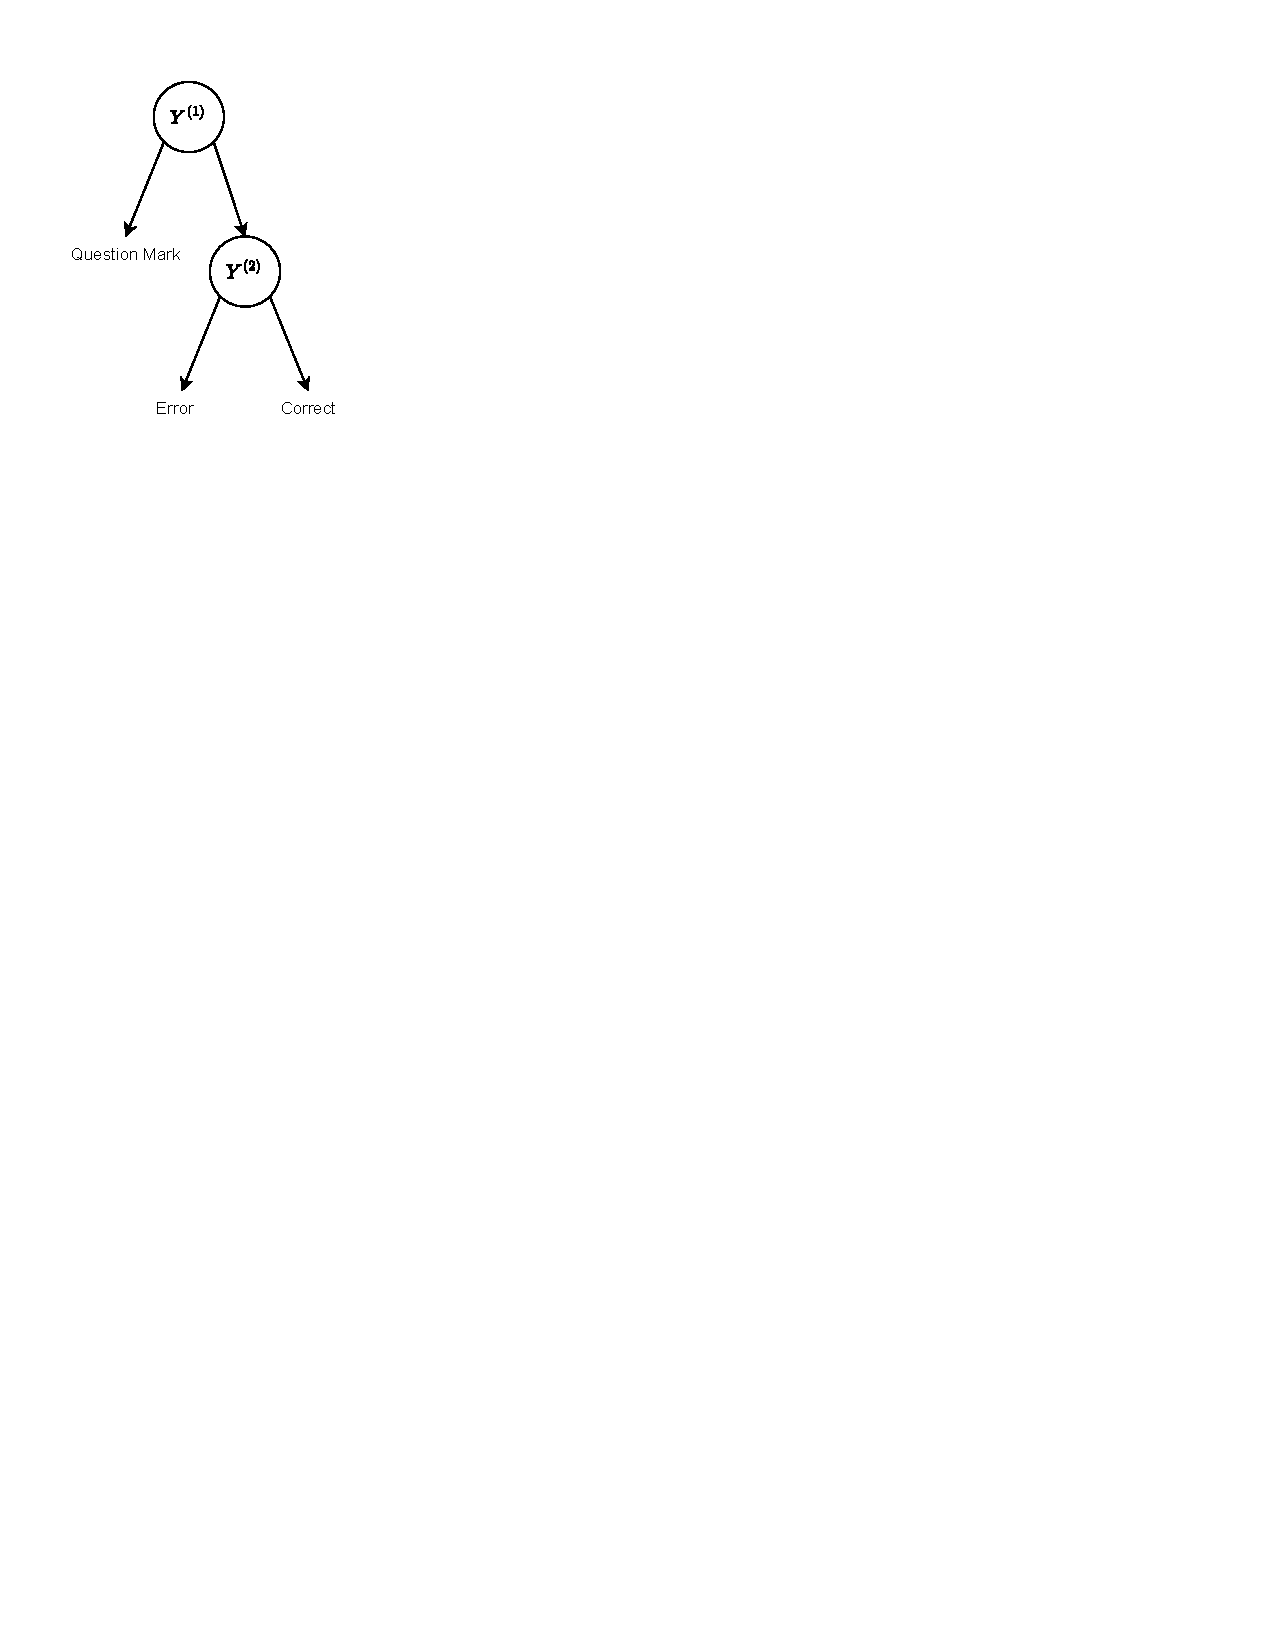
\includegraphics[width=0.3\linewidth]{figures/tree.pdf}
        \caption{A binary decision tree (IRTree model) with 2 nodes reflecting the decision to respond or not ($Y_1$) and whether the response is correct or not ($Y_2$).}
        \label{fig:tree}
\end{figure}


\subsection{Model Estimation and Comparison}
All models are estimated with the software package \textit{lme4}~\parencite{bates2015package} in R. 

To test the degree to which accuracy and problem-skipping represent the same or separate latent traits, we compare a baseline unidimensional model against three multidimensional models with varying constraints on the random effects. Table \ref{tab:model-comp} gives an overview of each model's parameter structure. The models range from fully multidimensional (random effects are estimated on both a person- and item level), to unidimensional (all responses are collapsed onto a single shared dimension).  

We compare these four models using Akaike Information Criterion~\parencite[AIC;][]{akaike2003new} and Bayesian Information Criterion~\parencite[BIC;][]{schwarz1978estimating}) values. However, these fit indices can perform less reliably when models differ in their random effects structure~\parencite{vaida2005conditional, greven2010behaviour}. We therefore also performed a 10-fold cross-validation. For each fold, 10\% of responses per student per node were held out, and the models were fitted on the remaining 90\%. Root mean squared error (RMSE) was computed on the held-out responses, which gives an indication of how well the model fit generalizes beyond the training data. 

\subsection{Data}
\subsubsection{Online Learning Environment}
% ANONYMOUS VERSION
We use data from an adaptive learning platform, [X] developed for primary school students to study Math and Language \footnote{In the current version of this manuscript, the name of the learning platform, and the country in which it is active, is hidden for anonymity. In places where the final manuscript would refer to the platform, the name has been replaced with [X].}. The platform currently consists of 65 games divided between environments designed for Arithmetic practice (28 games), language learning (24 games), and for second-language English learning (13 games). It is currently being used by over \num{450000} children across \num{4300} schools. Depending on the item format, the student needs to select one out of multiple answer options, or fill in the number themselves. They can skip the item by clicking a question mark. Then, the correct answer is shown and the student continues to the next item. While on the platform, children take care of a virtual garden, where each game represents a different learning domain, and the amount of practice is shown as the health of the plant. 

In this work, we use data from a game called Series (Figure~\ref{fig:series}), wherein a student is asked to fill in a missing number in a number sequence. This game is designed to test knowledge of number sequences and relations. Each item that a student completes is given a score, determined by a reward system~\parencite[for an overview, see][]{maris2012speed}, where the learner is shown coins that gradually disappear every second until the deadline (20 seconds). If the item is answered correctly, the amount of coins remaining is awarded, whereas if the answer is incorrect, the remaining amount of coins is lost. If the student skips the item or does not answer in time, no change is made to their score. 

Item difficulties and student abilities are estimated with the Elo Rating System~\parencite{elo1978rating}, which continuously updates student ability ratings, $\theta$, and item difficulty ratings, $\beta$, according to incoming data~\parencite{klinkenberg2011computer}. This ensures the adaptivity of the system: when a learner plays on the default medium difficulty setting, the system selects items with an expected probability correct of around 75\%. This probability changes to 90\% or 60\% if the student chooses to play on the easy or hard level, respectively. 

\begin{figure}[htbp]
    \centering
    % \begin{minipage}{0.5\textwidth}
        \centering
        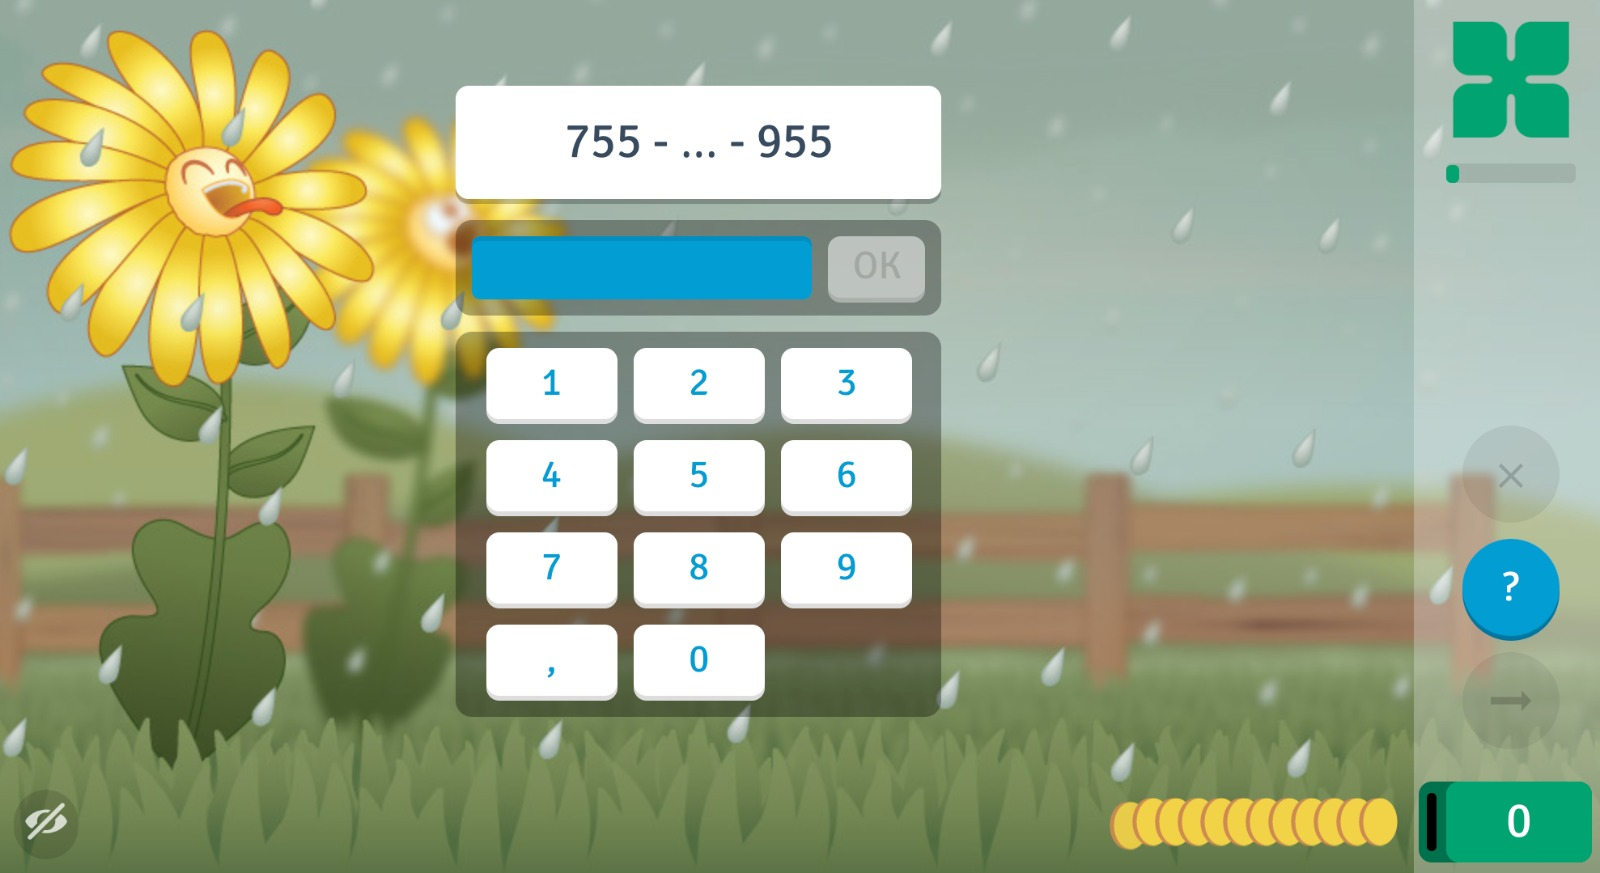
\includegraphics[width=.8\linewidth]{figures/series.jpeg}
        \caption{A screenshot of the Series game. A student is asked to fill in the missing number in the sequence. They gain (correct answer) or lose (incorrect answer) coins corresponding to the remaining amount of time in seconds (bottom right). A student can click the question mark (middle right) to retrieve the answer to the item and move on to the next.}
        \label{fig:series}
    % \end{minipage}%
    % \hfill % Add space between the figures
    % \begin{minipage}{0.5\textwidth}
    %     \centering
    %     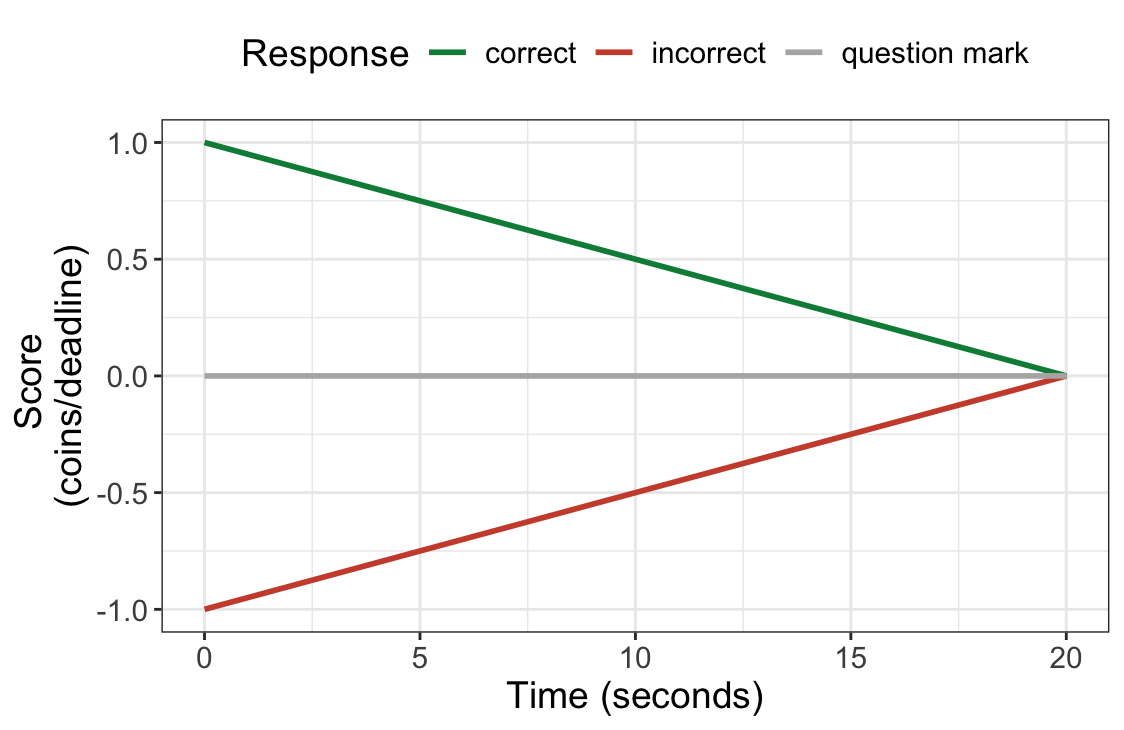
\includegraphics[width=\linewidth]{figures/scoringrule.png}
    %     \caption{Visualization of the explicit scoring rule.}
    %     \label{fig:scoring}
    % \end{minipage}
\end{figure}

\subsubsection{Inclusion criteria}
To obtain data suitable for the IRT fitting procedure we selected a specific subset of data from the Series game. First, we sampled data from the 2-year period between 01--09--2014 and 31--08--2016. In recent years, changes have been made to the reward system and the accessibility of the skip response in [X]. To ensure that these changes do not affect skip behavior in our analyses, we chose to look at data before this period of time. Lastly, the adaptive nature of the online learning environment means that user ability parameters are continuously updated. This also implies that for each user, there are periods of relative stable and unstable (denoted by jumps or shifts in learning) measurements of user ability. In order to control for possible effects of learning on problem-skipping, we only included data from periods where a user's ability remained relatively stable. We defined a stable period as one where the user's ability rating stayed close to their average rating within that period. Specifically, a stable period was when the user's ability rating did not fluctuate more than 1 rating point above or below their average rating\footnote{To this end we used the estimated ability rating from the online learning systems. This scale varies between -24.4 (min) and 15.9 (max), SD = 5.1)}. The average rating for each user was calculated by taking the 20\% trimmed mean of all their ability ratings, to prevent outliers from skewing the average. This criterion helps to minimize the influence of learning (or sudden jumps in ability) on skipping. Lastly, for proper identification of the models, we selected only users who had skipped a minimum of 10 responses within their data period. The length of each obtained period of learning data varied between users, with the mode around 1--2 weeks and the max up to 80 weeks.

On the item side, we selected items that had been played a minimum of \num{2000} times within the selected data collection period. The final dataset consisted of \num{3795} respondents and \num{386} items. 

\section{Results}
\subsection{Description of Problem-Skipping }
On average, children skipped approximately 6\% of items in the Series game. Our exploration of problem-skipping behavior revealed several trends. First, unsurprisingly, skipping was more common among children playing on the hard level ($M = 0.086, SD = 0.281$), compared to easy ($M = 0.043, SD = 0.203$) and medium ($M = 0.050, SD = 0.218$) levels. There was an interaction between grade and difficulty level: children playing on the hard level showed stable proportions of problem-skipping over all grades, whereas skipping decreased across grades on easy and medium levels (Figure~\ref{fig:grade_diff}). 

\begin{figure}[htbp]
      \centering
      
\includegraphics[width=0.8\linewidth]{BJET-26/figures/skip_grade.png}
      \caption{Proportion of skips in the Series game, separated by grade and difficulty level (easy = 90\% correct; medium = 75\% correct; hard = 60\% correct). Ribbons around the line denote the $95\%$ confidence interval. Grade refers to the Dutch grade levels; age ranges approximately between 4 and 12 years.}
      \label{fig:grade_diff}
\end{figure}  

We also found differences with regards to at what point in time skipping happened. Figure~\ref{fig:rt} displays the probability of each response type (correct, incorrect, skip) across response times. Problem-skipping was much more likely to occur in the first five seconds upon the presentation of an item, and very unlikely to occur after five seconds, though with a small increase in probability upon nearing the response deadline at 20 seconds. This is in stark contrast to the probability of making a correct response, which quickly increased in the first five seconds and slowly decreased leading up to the deadline. The probability of making an incorrect response showed a small peak early in the response process, and slowly increased with increasing response times. This figure also demonstrates that within the response times that are most common (where the histogram bars are the highest), the probability of skipping is relatively low. 

Similarly, with increasing number of items played in the Series game, the probability of skipping the problem shows an initial sharp decrease that gradually levels off, converging to a stable rate around the 25th item (Figure~\ref{fig:session}). This indicates that as users gain more understanding of how to play the Series game, their problem-skipping decreases. This graph also demonstrates the adaptivity of the system: as user ability estimates get more certain, the probability of making an error and skipping stabilizes. 

\begin{figure}[htbp]
    \centering
    \begin{minipage}{0.48\textwidth}
        \centering
        
\includegraphics[width=\linewidth]{BJET-26/figures/rt_dist.png}
        \caption{The probability of each response type (correct, error, skip) across response times (seconds). Point size refers to the amount of observations at that data point. The vertical line denotes the deadline to respond, at 20 seconds. The histogram displays the average distribution of response times in the Series game.}
        \label{fig:rt}
    \end{minipage}%
    \hfill
    \begin{minipage}{0.48\textwidth}
        \centering
        
\includegraphics[width=\linewidth]{BJET-26/figures/skip_session.png}
        \caption{The probability of answering with a skip or giving an incorrect response, over the first 100 items played in the Series game. Point size refers to the amount of observations at that data point.}
        \label{fig:session}
    \end{minipage}
\end{figure}



\subsection{Models of Problem-Skipping }
To test whether problem-skipping is distinguishable from accuracy in the Series game, we compared a fully estimated multidimensional response tree to a unidimensional response tree, and two versions of a multidimensional response tree where either random item effects (item-constrained IRTree) or random user effects (user-constrained IRTree) were constrained (full model specifications are highlighted in Section~\ref{section:analyses}). We compared these models on the basis of AIC and BIC model fit (Table~\ref{tab:model-comp}). The fully estimated IRTree model fit the data best, supporting the inclusion of a latent trait for problem-skipping in the estimation of student ability. 

The fully estimated IRTtree model had a fixed intercept of $-1.85$ ($p < .001$). This translates to a baseline probability of making an incorrect response of approximately $14.1\%$. Crucially, the correlation between the propensity to problem-skip (node 1) and give an incorrect response (node 2) was $0.41$: students that were more likely to problem-skip were moderately more likely to make erroneous responses. Although this correlation is positive, it is not 1 (which is the assumption under the unidimensional model). Similarly, the correlation between the item skipping threshold and item difficulty was $0.77$. That is, items that were more likely to be skipped were more likely to result in an incorrect response. The correlations between nodes for items and users is visualized in Figure~\ref{fig:cor}. 

\begin{table*}[t]
    \centering
    \small % Reduce font size for the table
    \begin{tabular}{p{1cm}p{3.5cm}ccccc}
        \hline
        \textbf{Model} & \textbf{Random Effects} & \textbf{AIC} & \textbf{BIC} & \textbf{RMSE} & \textbf{cor($\theta^{(1)}, \theta^{(2)}$)} & \textbf{cor($\beta^{(1)}, \beta^{(2)}$)} \\
        \hline
        1 & $\theta_p, \theta_i, \beta_p, \beta_i$ & 1519007 & 1519095 & 0.3217 & 0.41 & 0.78 \\
        2  & $\theta_p, \beta_p, \theta_i = \beta_i$ & 1533720 & 1533783 & 0.3234 & 0.35 & - \\
        3  & $\theta_i, \beta_i, \theta_p = \beta_p$ & 1550148 & 1550211 & 0.3251 & - & 0.73 \\
        4 & $\theta_i = \beta_i, \theta_p = \beta_p$ & 1566326 & 1566377 & 0.3268 & - & - \\
        \hline
    \end{tabular}
    \caption{Model fit statistics and latent correlation estimates for the four fitted models. RMSE = root mean square error. RMSE values were computed via $k$-fold cross-validation, where 10\% of the data was held out in each fold, the model was fit on the remaining data, and RMSE on the model predictions was calculated on the held-out set. The reported RMSE is the average across all folds.}
    \label{tab:model-comp}
\end{table*}


\begin{figure}[t]
    \centering
    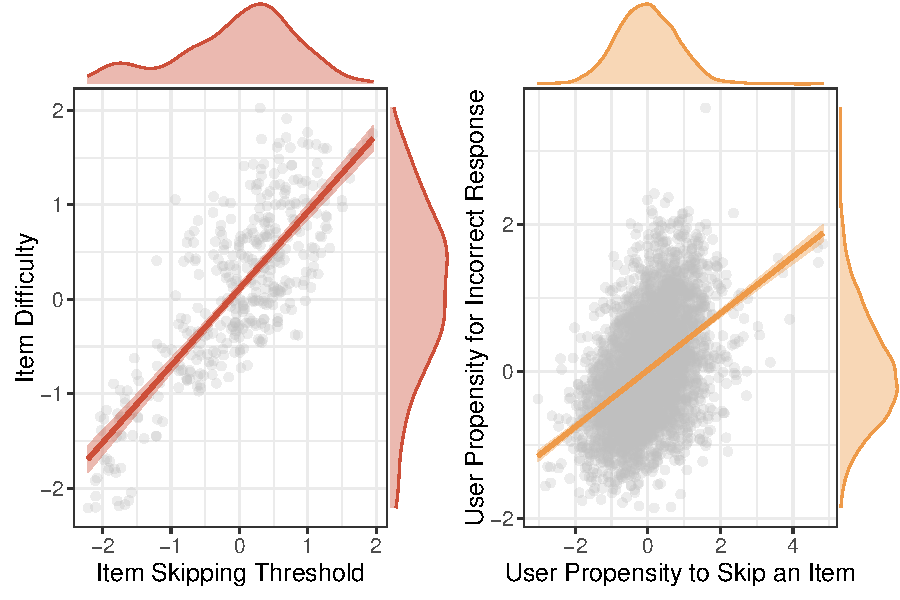
\includegraphics[width=0.8\linewidth]{figures/cor.pdf}
    \caption{Correlation between nodes in the fully estimated IRTree model. The left graph displays the correlation between the item skipping threshold ($\beta_{i, d=1}$), and the item difficulty ($\beta_{i, d=2}$). The right-hand graph displays the correlation between the individual propensity to skip an item ($\theta_{p, d=1}$), and the individual propensity to answer incorrectly ($\theta_{p, d=1}$). For both graphs, The scatter plot denotes individual data points, and the regression line displays the best-fitting linear relationship between the nodes. Density plots denote the distribution of each random parameter.}
    \label{fig:cor}
\end{figure}

\subsection{Individual Patterns in Problem-Skipping }
\begin{figure*}[t]
    \centering
    % 
\includegraphics[width=1\linewidth]{user_interactions.pdf}
    
\includegraphics[width=\textwidth,height=6cm]{BJET-26/figures/ind_responses_v09.png}
    \caption{Eight individual users extracted based on their estimated propensity to skip and make an incorrect response (center graph). Individual interaction patterns are displayed in a clockwise fashion starting from the upper right corner (low accuracy, high skipping), to the upper left corner (low accuracy, low skipping) of the scatter plot. Each graph plots each each individual's response sequence to items in the Series game. The position on the y axis reflects the response time to the item. Colors denote the response type (correct, incorrect, skip). While some users had longer response sequences in the extracted data (users C and E), the x axis is limited to showing the first 300 responses, to ease the visualization.
    }
    \label{fig:interactions}
\end{figure*}

In addition to indicating the average relationship between individual propensities to problem-skip and give an incorrect response, the scatter plot of user estimates in Figure~\ref{fig:cor} reveals the spread of data around this relationship. From this, it could be of particular interest to look closer at the play behavior of students that either conform to or deviate from the average pattern of problem-skipping and accuracy. Exploring individual patterns in problem-skipping could reveal further insights and generate new hypotheses about individual differences in interacting with online learning systems. To explore this, we randomly selected users from 4 sets of criteria: (1) Low accuracy and high skipping rate (upper right corner of the scatter plot); (2) High accuracy and high skipping rate (lower right corner of the scatter plot); (3) High accuracy and low skipping rate (lower left corner of the scatter plot); (4) Low accuracy and low skipping rate (upper left corner of the scatter plot). We visualized their interactions with items in the Series game by plotting their response type (correct, incorrect, skip) for each item across time, against their response time (Figure~\ref{fig:interactions}). This allows us to look at patterns in response types across time as well as whether responses were fast or slow and how this fluctuates. 

This exploration revealed some interesting patterns. For example, because user ratings cannot improve with a skip response, users with a high ability should, in theory, not resort to using the skip response at a high rate. When taking a closer look at these users (users C and D in Figure~\ref{fig:interactions}), they seem to be resorting to a different strategy compared to the other sampled users: long sequences of question-mark responding to avoid giving an answer, combined with sequences of attempting the item wherein the answer is mostly correct. In fact, the majority of users within this region of average skipping and accuracy showed such sequences, whereas the majority of users outside this region did not. 
 
\section{Discussion}
%% NOTES %%%%%%%
% I discuss the person-level correlation here, but the item-level correlation is not really discussed. A reviewer could question what the 0.77 item-level correlation implies? Perhaps the unidimensional model is a reasonable approximation for items? Is this relevant?

Adaptive learning technologies require accurate measurement models. In this study, we compared a unidimensional IRT model, which assumes that problem-skipping does not influence student ability differently from accuracy, to a multidimensional IRTree model, which explicitly accounts for differences in the propensity to skip an item. We found evidence that problem-skipping and ability are distinguishable processes, and as such, should not be measured on the same scale. Additionally, we found a moderate, positive association between problem-skipping and accuracy, suggesting that students with a high propensity to skip problems are somewhat more likely to be inaccurate when they do give a response. However, the relative weakness of this correlation opposes the assumption of unidimensional measurement models that these are perfectly correlated. Instead, it implies that skipped responses carry information about both accuracy and other meta-cognitive or motivational traits which affect responding. Failure to account for this will introduce bias to measurement and limit the adaptivity of the system; for a learner with a higher propensity to skip a unidimensional model would underestimate the ability to provide an accurate response.

Our findings extend previous work on response scale data and achievement test data---demonstrating that ignoring skipped items may lead to bias in the measurement of latent traits~\parencite{holman2005modelling, pohl2014dealing, huang2020mixture, okumura2014empirical, debeer2017modeling}---to online learning platforms. They also shed some light on the mixed evidence concerning the relationship between problem-skipping and accuracy, adding to the findings of~\textcite{norum2024student} that more problem-skipping is associated with more errors, and the body of literature indicating individual differences in the use of alternative response options~\parencite{norum2024student, goldin2012learner, goldin2013hints}. However, the evidence that problem-skipping and accuracy are distinct and only moderately related may also help to explain the discord in the literature. Specifically, the imperfect relationship suggests that the observed association between problem-skipping and accuracy may be influenced by contextual factors, such as the design of the learning environment or task difficulty, which give space for different manifestations of meta-cognitive strategies and motivational states such as frustration or boredom. Future work should aim to disentangle these contextual influences to better understand the role of problem-skipping in learning and assessment. 

Many adaptive learning platforms include a response option alternative to directly attempting an item, such as skipping the item or requesting a hint. These findings, therefore, have relevance for any ALS that aims to provide a fair estimate of student ability while allowing flexibility in how students engage with items. A basic recommendation for such systems is to, at a minimum, measure both latent traits once the data have been collected. The IRTree model has proven a feasible method for this kind of post-hoc analysis, offering insights into individual differences in both accuracy and problem-skipping. However, there are some limitations to the use of IRTree models: they require large amounts of data for reliable estimates, making them less suitable for students who interact with the learning platform less frequently. Moreover, in the way that it is currently implemented, this method reflects past behavior rather than providing real-time insights, a core feature in ALSs. In practice, the IRTree framework could be used to incorporate a second parameter into the measurement model for real-time tracking of problem-skipping. This would enable adaptive systems to monitor and act on these tendencies as they emerge, for example via teacher dashboards. While this method is still data-intensive, it would allow for dynamic tracking of both accuracy and problem-skipping, providing a fuller picture of the learning process. 

Despite their importance in revealing individual differences in how problem-skipping relates to accuracy, post-hoc and real-time models reveal little about where these differences stem from. This raises the question of whether different types of meta-cognitive strategies or states---such as boredom, frustration, gaming, or wheel-spinning---can be inferred from students' response data. Consider two students, one of whom quickly skips items in a very long sequence (students C and D, Figure~\ref{fig:interactions}) to avoid effort, and another who is exerting effort into learning by attempting as many items as they can, but skips the item as soon as they are uncertain to avoid the risk of negative feedback. While both students would display high problem-skipping tendencies, they bode for different intervention styles and may therefore want to be separated. To aid in this, more information can be added to the tree model, such as a node to distinguish fast from slow responses~\parencite{coomans2016distinguishing, hofman2018fast}. An IRTree model can also be extended to model different levels of disengagement, by, for example, explicitly accounting for drop-out~\parencite{huang2020mixture}. 

Apart from merely measuring different cognitive and meta-cognitive states from observed response data, adaptive systems can be designed to make these strategies directly observable. One approach is to provide response options explicitly linked to meta-cognitive strategies, allowing systems to infer and adapt to the strategies students employ. The feasibility of such an approach would depend on the scale and flexibility of the learning system. For instance, in a system with an exploratory style of learning, mapping response options to every possible strategy may prove challenging. An alternative approach is to change the reward structure of the environment in such a way that it constrains students' behaviors to a specific strategy. For example, if problem-skipping is seen as undesirable behavior---such as indicating low effort or gaming the system---the reward structure of the system can be changed in such a way that this behavior is decreased. Such an intervention has been successfully implemented, wherein the ability to use the problem-skipping option was delayed upon the presentation of each item~\parencite{savi2018delaying}. This led to an increase in the amount of items that students attempted, promoting effortful responding in the system. Such interventions highlight the potential of system design to nudge students toward more productive behaviors.

%For example, in [X], a reward system~\parencite{maris2012speed} is implemented in such a way that students are challenged to provide adhere to a speed-accuracy trade-off. In a similar manner, a separate reward structure for problem-skipping can be implemented such that it has an appropriate trade-off with accuracy known to the learner. A potential future research avenue is to investigate the applicability and validity of such approaches for detecting different problem-skipping strategies. 

%Lastly, if problem-skipping is seen as undesirable behavior---such as indicating low effort or gaming the system---the design of the system or scoring rule can be changed in such a way that this behavior is decreased. Such an intervention has been successfully implemented, wherein the ability to use the problem-skipping option was delayed upon the presentation of each item~\parencite{savi2018delaying}. This led to an increase in the amount of items that students attempted, promoting effortful responding in the system. Such interventions highlight the potential of system design to nudge students toward more productive behaviors.

A final note to consider is that while the fully multidimensional model shows that problem-skipping and accuracy are governed by separate processes, it does not shed light on the true decision process of the student. In the future, it would be interesting to compare different modeling frameworks aimed at deciphering the decision process more explicitly. For example, Race Models~\parencite{heathcote2022winner} assume that there is competition between two or multiple parallel processes, and as enough evidence accumulates in support of one process, this process wins and determines the subsequent decision. In the context of problem-skipping, such a model may be suitable for detecting fine-grained processes such as individual differences in processing speed, especially in the context of a speed accuracy trade-off~\parencite{heathcote2022winner, evans2018modeling}. Alternative methods to model students' decision-making processes include Bayesian Hierarchical Models~\parencite{sawyer2018modeling, lee2014bayesian} and Markov Decision Processes~\parencite{lamar2018markov, puterman1994markov}. The rich, granular data generated by online learning systems offer an ideal opportunity to compare cognitive decision models, which usually require detailed and structured data collected in lab experiments. Nevertheless, the current results already indicate that there are structural individual differences which, regardless of how the process is modeled, needs to be accounted for.

%\vspace*{2em} % add if header hovers alone at end of page in final version
\section{Conclusion}
In a large-scale adaptive learning environment for arithmetic practice, we found that accuracy and problem-skipping are moderately related, but distinct traits. Under a measurement model which doesn't explicitly account for individual differences in problem-skipping, student ability estimates could disadvantage children who respond differently to problem-skipping options. To prevent this, online learning environments should consider estimating and reporting latent traits for both the tendency to problem-skip and give an accurate response, or intervene in the learning system such that strategies can be inferred or problem-skipping is reduced. We have shown the feasibility of applying the IRTree framework~\parencite{de2012irtrees} to model problem-skipping in an adaptive learning platform. We believe this approach has the potential to be extended to model other response strategies and learning contexts. Only with accurate measurement models can equity in learning analytics be realized. 

\section{Data and Code Availability}
The dataset used in the current study was collected under license of the third party company to which the data belongs. Restrictions apply to the availability of these data, but can be made available from the authors upon reasonable request and with permission of the company. Source code used to fit and analyze the data is publicly available at [github repo].

%\bibliographystyle{apaparencite}
%\bibliography{qm_bib} 
\printbibliography

\end{document}
